\documentclass[journal]{IEEEtran}

\usepackage{graphicx}

\usepackage{booktabs}

\usepackage{array}

\usepackage{url}

\title{A Synthetic Benchmark for Dairy Cow Health Monitoring With a Hybrid LSTM-XGBoost Prototype}

\author{Author name and affiliation to be supplied}

\begin{document}

\maketitle

\begin{abstract}Dairy health monitoring can combine wearable sensing with machine learning, but early prototypes are often evaluated before a representative clinical dataset is available. This study builds a reproducible synthetic benchmark and a local farmer-facing dashboard to examine one such workflow. We generated 10,000 daily records for 150 synthetic cows, with 14.73% assigned a sick label. Three-day windows were split by cow, leaving 2,890 windows from 45 cows for an untouched test set. A 32-unit long short-term memory encoder produced a 16-dimensional embedding, which was fused with temperature-humidity and forage indicators and classified by XGBoost. On the synthetic holdout, the hybrid achieved 99.69% accuracy, 99.06% precision, 98.83% recall, 98.94% F1, 0.16% false-positive rate, and 99.72% area under the receiver operating characteristic curve. A raw-feature XGBoost comparator achieved 99.62% accuracy and 98.71% F1. These scores describe a controlled synthetic-data experiment, not field performance: labels were sampled first and sensor features were then generated conditionally from those labels. The dashboard also displays synthetic readings and a transparent heuristic rather than predictions from a validated clinical model. The results support a reproducible software demonstration, while real-world deployment requires prospective sensor data, veterinary labels, external validation, and a secured data service.\end{abstract}

\begin{IEEEkeywords}dairy cattle, precision livestock farming, synthetic data, LSTM, XGBoost, SMOTE, IoT dashboard\end{IEEEkeywords}

\section{Introduction}

A dairy cow may change its activity, rumination, pulse, or temperature before a worker sees an obvious clinical sign. Wearable collars can make these changes visible more often than manual checks, and networked systems can route readings to a shared dashboard. Kaur and Virk [1] describe a collar-based monitoring study that collected temperature, pulse, and accelerometer readings from 150 cows across seven districts in Punjab. Their work gives a practical starting point for a software prototype: sensor measurements must become a clear sequence of data, a cautious risk signal, and an action that a farmer can review.

This paper follows that path with a synthetic experiment. We generate daily records for 150 synthetic cows, form three-day windows, train a hybrid long short-term memory (LSTM) and XGBoost classifier, and place sample herd readings in a farmer/admin dashboard. The experiment asks whether the requested software pipeline can be implemented reproducibly and whether the model separates the synthetic labels under a cow-held-out split. It does not ask whether the model can diagnose disease on a real farm.

The central result is deliberately qualified. The hybrid scores are high on the synthetic holdout, but the generation process first samples the health label and then shifts sensor distributions according to that label. This makes the target easier to infer than an independently observed veterinary outcome. We therefore treat the score as a software and data-pipeline check, not evidence of clinical accuracy. The paper contributes a complete synthetic workflow, a no-LSTM XGBoost comparison, a role-separated local dashboard, and an explicit account of what must change before field evaluation.

The practical value of a monitoring system depends on more than its classifier. A useful workflow must preserve cow identity, attach a trustworthy time to every measurement, show a worker why an alert appeared, and allow the worker to check the animal. A model score without this context can create extra work or false reassurance. For that reason, this study treats the dashboard as part of the end-to-end prototype, while keeping its status separate from the model evaluation.

The study has three questions. First, can the requested sequence encoder and tree classifier be trained with an untouched cow-held-out test set? Second, how do its six reported metrics compare with a raw-feature tree model and with published values from [1]? Third, what data and safety steps would be needed before a farm trial? The answer to the first two questions is numerical but confined to the data generator. The third is a deployment plan, not a claim that the prototype is ready for use.

A farmer-facing system has a longer chain of dependencies than a model benchmark. A collar must remain attached, sensors must produce plausible values, a gateway must transmit them, and software must preserve their identity and timestamp. A missing signal can look like a healthy signal if the system silently carries forward an old measurement. The interface therefore needs to distinguish a current reading from a stale or absent reading. These reliability questions are outside the generated experiment, but they shape the system requirements for a future field study.

The intended use considered here is an early review prompt. It is not diagnosis or autonomous treatment. This distinction affects model design: the event threshold should reflect the cost and urgency of a veterinary check, and the user should be able to review the underlying measurements. The prototype helps make this intended interaction concrete, while the paper separates a software demonstration from evidence about animal health.

\section{Related Work}

Kaur and Virk [1] describe an IoT neck collar for dairy-cow monitoring and report Random Forest performance on their field dataset. Their study motivates the sensor context here, but its measurements, labels, and evaluation protocol differ from this controlled demonstration. Reviews of dairy-farm sensors and monitoring systems describe the broader move toward integrated health management and emphasize data quality and practical validation [14], [16].

Activity and behavior streams can add context to physiological measurements. Work linking activity-sensor data with cow physiology illustrates the value of interpreting movement in relation to animal state [11]. Wearable accelerometers have also been reviewed for measuring lying behavior, and collar validation studies show why the precision of the measurement itself must be checked before using it as a health signal [15], [18]. These sources motivate our inclusion of activity and rumination-related variables, while the present dataset does not reproduce validated sensor measurements.

Locomotion is another relevant signal for health monitoring. Reviews describe accelerometer-based lameness detection [13] and computer-vision approaches to dairy-cow lameness [12]. The gait-asymmetry feature in this study is only a generated proxy; it is not a measured gait score and cannot establish clinical lameness. A future field study would need reference labels and on-farm validation.

Deployment depends on the setting as well as the sensing method. A survey of sensor systems used on Italian dairy farms reports variation in the systems used and the herds that adopt them [16]. Adoption research identifies practical factors affecting precision-monitoring uptake [17]. The dashboard in this bundle is therefore presented as a local software demonstration, not an operational farm service.

For modeling, SMOTE interpolates minority-class examples in feature space [2], while LSTM networks provide a gated mechanism for learning from ordered inputs [3]. XGBoost is a gradient-boosted tree system used here for the final classifier [4]. Class imbalance makes accuracy alone an incomplete summary; ROC analysis [5], precision-recall behavior [6], and the broader imbalanced-learning literature [7] motivate reporting multiple metrics.

The evaluation design also follows the principle that data with hierarchical or temporal structure requires an appropriate split strategy [8]. Transparent reporting guidance supports documenting the intended use, data, and analysis choices [9], while calibration is a separate property from discrimination and should be checked before presenting model scores as probabilities [10]. These methods inform the prototype, but do not substitute for independent clinical validation.

\section{Synthetic Dataset}

The generator creates exactly 10,000 daily records and assigns each record to one of 150 cow identifiers. A seeded random process marks 1,473 records as sick and 8,527 as healthy, giving 14.73\% sick prevalence. The nine input fields are cow\_id, avg\_temp, avg\_pulse, avg\_activity, rumination\_slope\_6h, gait\_asymmetry, THI, ventilation\_index, and forage\_index. The target is binary. The variables were selected to extend the temperature, pulse, and activity signals in [1] with rumination, gait, and environmental context.

The activity field is a noisy ordinal category from 1 to 3. It echoes the mild, moderate, and intense activity categories discussed by Kaur and Virk [1], but the generator does not reproduce their accelerometer magnitude and threshold calculation. Temperature, pulse, rumination slope, and gait asymmetry are sampled from distributions shifted by the synthetic label. THI is uniform from 60 to 85; ventilation and forage indices are bounded between zero and one. Environmental stress adds small shifts to selected variables.

For each cow, the records are ordered by their synthetic sequence and the first two records are used only as warm-up context. This yields 9,700 three-day windows. There are no observed calendar dates or real sensor traces. The windows therefore represent a controlled sequence shape, not authentic consecutive days. Table I summarizes the synthetic classes and feature groups.

Table I groups the fields by role. Cow identity is included in the model input as requested, but it is an identifier rather than a physiological measurement. This choice has a consequence: a real deployment should test whether identifier information helps only because of data artifacts. The cow-held-out partition reduces direct memorization of identifiers across the two sets, but it does not establish that cow identity is a useful predictive signal. A sensitivity analysis excluding cow\_id would be appropriate on collected data.

The generator samples each day's health label first, with a Bernoulli probability of 0.15. It then samples environmental indicators and creates health-related measurements conditional on that label. Temperature is centered near 38.85 degrees for healthy records and shifted upward by 0.95 degrees for sick records, with a small heat-stress adjustment. Pulse is centered near 65 beats per minute for healthy records and shifted upward by 23 beats per minute for sick records. Activity is an ordinal category formed by rounding a noisy score and clipping it to one through three. Rumination slope and gait asymmetry are also shifted for sick records. Values are clipped to stated operating ranges where applicable.

The exact row count is fixed at 10,000, and the target draw produced 1,473 sick records in the saved seed-42 dataset. The CSV in the package contains the full analysis records and metadata columns for cow assignment and within-cow order. The model uses only the nine named input fields; target is used as the label, while row-order metadata supports the sequence construction and is not a predictor. This separation is important for reproducing the reported experiment.

These values are designed for a controlled software benchmark and are not fitted estimates of farm distributions. For example, the simulator does not reproduce sensor calibration, missing readings, device drift, medication effects, lactation stage, parity, breed, or co-occurring disease. It also does not model a clinically meaningful onset process. Adjacent rows in the generated order are used as three-step context, but the rows are not linked to real calendar dates. The saved dataset therefore allows code review and repeatable analysis, not epidemiological inference.

The feature ranges are interpreted as broad interface-oriented ranges rather than validated biological reference intervals. Temperature is clipped from 37 to 42 degrees, pulse from 35 to 150 beats per minute, gait asymmetry from zero to one, and ventilation and forage indices from zero to one. THI is drawn between 60 and 85. Activity is encoded as an integer from one to three. Rumination slope is not clipped, so its range follows the generated distribution. Units and collection intervals for the added features would need a formal data dictionary before collecting real measurements.

Environmental context is represented by a simple heat-stress term derived from THI. Values above 72 increase the expected temperature and pulse and slightly lower activity and rumination. Ventilation and forage are generated from beta distributions that favor mid-to-high values. They are not used to create a veterinary outcome; rather, they supply plausible bounded context fields for the data table. The target-dependent shifts in the physiological and behavioral measurements remain the dominant source of separability.

The fixed seed supports exact reproduction of the saved dataset under compatible library behavior. The data-generation script stores a per-row original order and a within-cow index. The analysis CSV retains the cow identifier, day index, input features, and target, while the internal ordering field used during generation is removed from the distributed CSV. The order field allows a reader to inspect how sequence windows were assembled, but no calendar timestamp is claimed. Reproducing a row split without the original ordering would not recreate the exact windows, so the package also includes the executable generator.

A useful extension would preserve an explicit data lineage file containing the random seed, generator version, date of generation, and feature schema. In a farm collection, lineage would include sensor firmware, calibration records, and a mapping from device identifier to animal identifier. Such records help explain whether a later change in model output comes from animal behavior, device changes, or preprocessing. The present project does not include a sensor device, but its schema can serve as a starting point for that documentation.

\begin{figure}[!t]\centering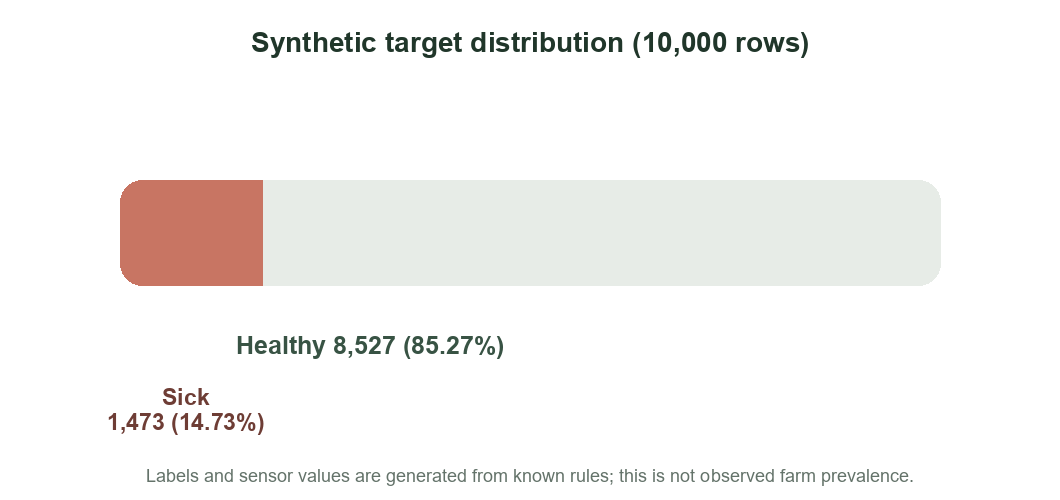
\includegraphics[width=\columnwidth]{../figures/class_distribution.png}\caption{Synthetic class prevalence; labels are synthetic.}\label{fig:classes}\end{figure}

\begin{table}[!t]\centering\caption{Synthetic data summary}\begin{tabular}{p{0.95in}p{1.9in}}\toprule Item & Description \\\midrule Records and labels & 10,000 rows; 8,527 healthy and 1,473 sick \\ Cow identifiers & 150; random assignment with replacement \\ Physiological & Temperature and pulse \\ Behavioral & Activity, rumination slope, gait asymmetry \\ Context & THI, ventilation, forage \\ Identifier input & Numeric cow identifier \\\bottomrule\end{tabular}\end{table}

\section{Model And Evaluation Design}

We split the 150 cow identifiers into 105 training cows and 45 test cows using seed 42. All windows from a cow remain in one partition. The resulting test set contains 2,890 windows, including 427 sick windows, for 14.78\% prevalence. Training preprocessing is fit without using the test set. SMOTE [2] balances flattened training windows before LSTM fitting. The trained encoder maps each three-step, nine-feature sequence to 16 values. We concatenate that embedding with the final record's THI and forage index and apply SMOTE again to the fused training vectors. No test sample is resampled.

The LSTM contains 32 recurrent units and a 16-unit ReLU embedding layer. A sigmoid classification head is trained with Adam and binary cross-entropy for up to ten epochs, with early stopping based on a 10\% validation slice of the resampled training windows. XGBoost uses 250 estimators, maximum depth 4, learning rate 0.05, row and column subsampling of 0.9, and seed 42. Its scale\_pos\_weight is computed from the resampled labels; because SMOTE balances those labels, the resulting ratio is one.

The no-LSTM comparator is an XGBoost classifier trained on the nine raw daily input features from the original, unresampled training windows. It uses the same cow-held-out split, estimator settings, and an inverse class-frequency scale\_pos\_weight. Predictions use a probability threshold of 0.5. Accuracy, precision, recall, F1, false-positive rate (FPR), and area under the receiver operating characteristic curve (AUC-ROC) are calculated on the untouched test set. We also report confusion counts so the small number of errors is visible. Fig. 2 summarizes the workflow.

The cow split is applied after three-day windows have been built. The 150 identifiers are partitioned into 105 training cows and 45 test cows. Each available window for an identifier follows that identifier into one side only. This prevents a direct overlap of a cow between training and test windows. It does not prevent the same label-dependent generator rules from appearing in both groups, which is why a high score remains expected under this construction.

A standard scaler is fitted only on the training windows and then applied to both partitions. Training windows are flattened for SMOTE and reshaped to three timesteps after resampling. The LSTM receives a window with shape three by nine and returns a 32-unit recurrent state. A dense 16-unit ReLU layer forms the temporal embedding, and a sigmoid head is used to train the encoder with binary cross-entropy. Early stopping monitors a validation slice drawn from the resampled training set. The XGBoost stage receives the embedding plus the final window's THI and forage index. The test side is kept at its original class prevalence and is never oversampled.

The comparator receives the nine raw features from the target day. It is fitted on the original, unresampled training rows, with scale\_pos\_weight set from the training class ratio. This comparison is useful as a software baseline, but it is not a controlled ablation of one component alone: training representation and imbalance handling differ between the hybrid pipeline and the comparator. A future ablation should hold these choices constant where possible and isolate the effect of the sequence encoder, environmental fusion, and resampling separately.

For a binary label, accuracy is the fraction of all test records classified correctly. Precision is the fraction of predicted sick records that are labeled sick, and recall is the fraction of labeled sick records detected. F1 is the harmonic mean of precision and recall. FPR is the fraction of healthy records incorrectly flagged, calculated as FP divided by FP plus TN. AUC-ROC measures ranking across probability thresholds rather than performance at only the 0.5 operating point. These quantities answer different questions and should be read together.

The model threshold is fixed at 0.5 for the reported confusion counts. It is not selected from a farm utility analysis. In practice, missed illness and unnecessary checks may have different costs depending on the farm, disease, staffing, and follow-up capacity. Any operational threshold must be selected using prospective data and reviewed with veterinary staff. Sensitivity, specificity, confidence intervals, calibration, and alert burden should be considered alongside the six requested summary metrics.

Sequence construction yields 9,700 windows because the first two available rows for each cow serve as context only. This is a mechanical consequence of three-step windows, not a claim that all animals have a continuous three-day monitoring history. The data generator assigns cows with replacement, so the number of rows per cow varies. Every window is assigned to the cow that contributes its final record, and all windows for an identifier remain in one split. A production pipeline would need to define what happens when a time step is missing or arrives late.

The final window step supplies the THI and forage indicators for fusion with the embedding. This choice makes the static fields align with the target-day record. The other seven raw features enter through the sequence representation. The encoder is trained using a sigmoid output head, but the separate XGBoost model performs the final reported hybrid classification. The neural head provides a supervised learning signal to the embedding; it is not the model used to produce the final hybrid probabilities. This distinction matters when reproducing the pipeline or interpreting the stage-specific feature importances.

Oversampling takes place at two points in the hybrid workflow. The training sequences are balanced before fitting the LSTM. The encoder's embeddings for the original training windows are then combined with the two context fields and SMOTE is applied to that fused training set before fitting XGBoost. The resampled sequence batch used for encoder training and the fused-vector set used for tree training therefore serve different stages. The test window array and test labels are never supplied to SMOTE. The saved final test set is the original unbalanced subset, not a resampled copy.

The reported AUC-ROC is calculated from the probability output, while the confusion counts and threshold-dependent metrics use a probability cut at 0.5. This avoids conflating ranking quality with a chosen operating point. The accuracy denominator is all 2,890 test windows. Precision uses predicted positives, recall uses actual positives, and FPR uses actual negatives. In this result, the 427 positive cases and 2,463 negative cases sum to the full holdout. The confusion matrices make these denominators inspectable rather than leaving the reader with percentages alone.

Metric interpretation should consider prevalence. Precision can change when the proportion of sick windows changes even if sensitivity and specificity remain stable. Therefore, the 99\% precision observed here is tied to the simulator's test prevalence and label construction. It cannot be transferred to a farm with a different disease rate. An operational study should report positive and negative predictive values at the observed prevalence and may include scenario analysis across plausible prevalences, while clearly labeling any prevalence-adjusted values as calculations rather than observations.

\begin{figure}[!t]\centering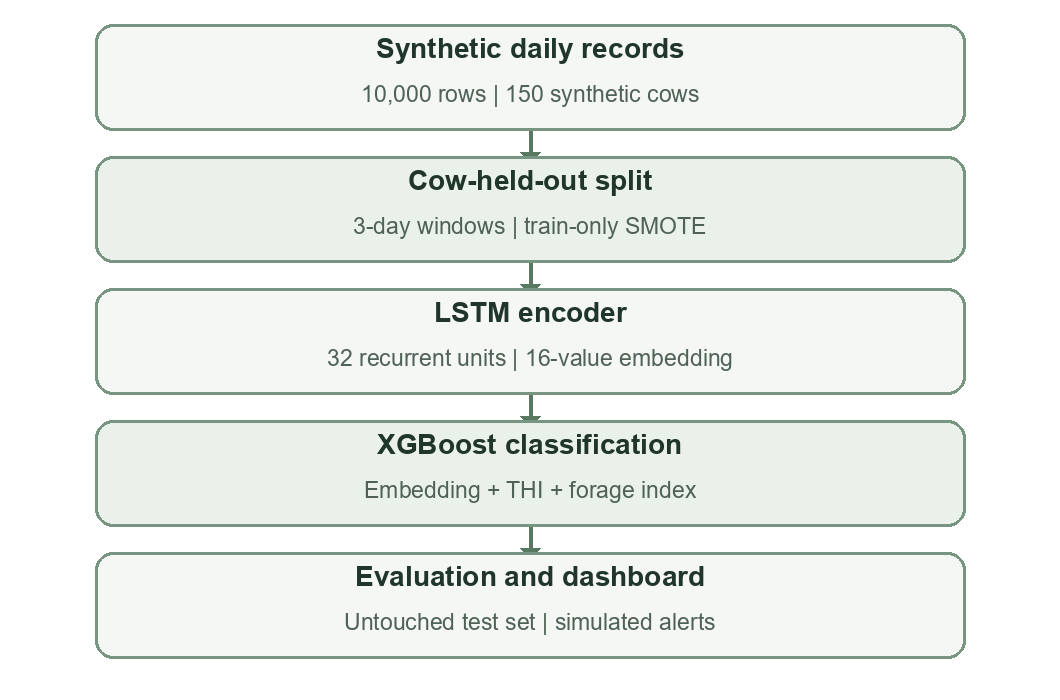
\includegraphics[width=\columnwidth]{../figures/workflow.png}\caption{Cow-level split, hybrid classifier, and demo dashboard path.}\label{fig:workflow}\end{figure}

\section{Farmer And Admin Dashboard}

The dashboard presents herd size, healthy/watch/attention counts, sensor summaries, risk ordering, and alerts. A polling endpoint advances a small synthetic sensor batch every five seconds. A farmer role can read herd and alert data; an administrator can also acknowledge an alert. In the local FastAPI demo, temporary credentials are generated at startup and the session is held in memory. The standalone server is intended for loopback testing, not public deployment.

The public GitHub Pages preview is a separate static page. It creates its own synthetic readings in the browser and has no server-side login, database, or protected write operation. GitHub Pages cannot host the FastAPI backend. The dashboard's displayed risk score is a transparent heuristic in the demo feed, not output from the trained LSTM-XGBoost classifier. These boundaries keep a visual prototype from being mistaken for a production monitoring service.

In the local demonstration, the interface is backed by a small FastAPI service and in-memory state. The farmer role is read-oriented, while the administrator role includes an alert acknowledgement action. The service exposes a health check and versioned API paths for login, herd readings, summary counts, and alerts. Access-control tests in the software project check that protected routes reject unauthenticated requests and that the farmer cannot use the administrative acknowledgement action. These controls are suitable for a local demonstration only; they are not a substitute for an audited identity system, persistent event log, transport security, or operational monitoring.

The static GitHub Pages version is intentionally different. It creates browser-side readings and refreshes them on a timer. A public static site cannot safely hold private credentials or enforce a role-based write operation. It is useful as a portfolio preview of the interface, but all data must be treated as public demonstration content. A real service would require a separate authenticated backend, a protected network connection, a database with retention rules, and access policies appropriate to farm records.

The monitoring view is organized around herd status, a sortable reading list, and recent alerts. This arrangement is intended to answer three immediate questions: how many animals need review, which cow should be checked first, and which measurements contributed to the displayed status. A production version should show the time of the latest received measurement and make data quality visible. If the latest update is stale, the system should not present it as a live reading. The current demo updates sample rows on a timer and should not be read as proof of network or sensor reliability.

An acknowledgement is an administrative workflow event, not a clinical outcome. A complete system would distinguish acknowledgement, examination, confirmed condition, follow-up, and resolution. Those states support auditing and allow analysts to evaluate alert usefulness. The local demo keeps state in memory and resets it after restart, so it cannot provide a reliable audit trail. Persistent storage and identity controls would be necessary before the interface could be used in an operational setting.

A local admin and farmer role separation is helpful for demonstrating access boundaries, but a role name alone does not provide security. The server must check authorization on every protected request, expire or revoke sessions, limit repeated login attempts, and avoid revealing sensitive information in error messages. A public Pages preview has no such server controls. It should contain only synthetic example values and public documentation. These distinctions are included so that readers do not confuse a static portfolio display with an authenticated farm service.

\section{Results}

The hybrid model classified 2,881 of 2,890 test windows correctly. It produced 422 true positives, 2,459 true negatives, four false positives, and five false negatives. Accuracy was 99.69\%, precision 99.06\%, recall 98.83\%, F1 98.94\%, FPR 0.16\%, and AUC-ROC 99.72\%. The no-LSTM XGBoost comparator produced 2,879 correct predictions, with 422 true positives, 2,457 true negatives, six false positives, and five false negatives. Its accuracy was 99.62\%, precision 98.60\%, recall 98.83\%, F1 98.71\%, FPR 0.24\%, and AUC-ROC 99.99\%.

On this synthetic partition, the hybrid had slightly higher accuracy, precision, and F1 than the raw-feature XGBoost model, while the XGBoost model had a higher AUC-ROC. The difference is small and cannot establish a general advantage. Figs. 3 through 8 show each evaluation metric separately. Table II reports the main scores, Table III reports FPR and AUC-ROC, and Table IV gives the confusion counts.

For context, Kaur and Virk [1] report a Random Forest result of 92.46\% accuracy, 92.36\% precision, and 92.36\% F1; their reported XGBoost result is 85.91\%, 58.59\%, and 73.72\%, respectively. Those values used the paper's own dataset and protocol. They are not matched baseline runs and are not plotted beside our synthetic results as if they came from a common test set.

At a threshold of 0.5, the hybrid model made nine errors among 2,890 test windows. The raw-feature XGBoost model made eleven. Both models detected 422 of the 427 positive test windows, so their recall is the same to the reported precision. The hybrid reduces false positives from six to four, a difference of two cases on this single partition. The lower FPR is therefore directionally favorable but based on a small count; it should not be presented as stable evidence of a general advantage.

Accuracy is high for both models because the synthetic test set contains more healthy than sick windows, but accuracy alone conceals the error pattern. Precision is slightly higher for the hybrid, while recall is equal. F1 summarizes that balance at the chosen threshold. The raw-feature model has the higher AUC-ROC even though its thresholded F1 is lower. This is possible because AUC-ROC evaluates ranking over all thresholds, whereas F1 uses one fixed threshold. The six charts in Fig. 3 through Fig. 8 show each metric separately and use only available values for each comparison.

Published Kaur and Virk values are included in the accuracy, precision, and F1 charts for context, while recall, FPR, and AUC-ROC are marked as unavailable where the paper does not report them in the cited comparison. The published Random Forest achieved 92.46\% accuracy and 92.36\% precision and F1; the published XGBoost achieved 85.91\%, 58.59\%, and 73.72\%, respectively [1]. Since the data, label definition, sampling, and test protocol differ, a visual juxtaposition is descriptive only. It is not a head-to-head benchmark.

Table II reports the scores to two decimal places for readability; the full floating-point values are preserved in data/results.json. Table III isolates FPR and AUC-ROC, and Table IV provides integer confusion counts. The six charts accompany the metrics rather than replacing the tables. Accuracy, precision, and F1 charts include values available from the cited paper [1]. Recall, FPR, and AUC-ROC charts contain only the models for which this paper reports a value, because the cited baseline does not provide comparable values for those measures in the referenced result. This avoids inventing missing scores.

The comparison across metrics is consistent with the confusion counts. Both models correctly identify 422 positive windows and miss five. The hybrid has four false positives; the raw-feature model has six. As a result, recall is identical, precision and F1 are marginally higher for the hybrid, and FPR is marginally lower. The XGBoost raw-feature AUC-ROC is higher because its probabilities rank the holdout labels slightly better across thresholds even though its 0.5 predictions include two additional false positives. Small absolute differences should be interpreted against the single-split design and the generator's strong label signal.

The published Random Forest and XGBoost values are useful as a reference point for the research context, not as an external validation set. Their chart bars are included with a note on protocol differences. A visual comparison can make the scale of reported values easy to understand, but it can also suggest a contest that the data do not support. The manuscript therefore describes the source and limitation next to the charts and does not claim that the hybrid outperforms the paper's Random Forest.

\begin{table*}[!t]\centering\caption{Model results in percent. Values from [1] use a different dataset and protocol.}\begin{tabular}{l r r r r}\toprule Model & Accuracy & Precision & Recall & F1 \\\midrule Hybrid LSTM-XGBoost & 99.69 & 99.06 & 98.83 & 98.94 \\ Raw-feature XGBoost & 99.62 & 98.60 & 98.83 & 98.71 \\ Random Forest [1] & 92.46 & 92.36 & NR & 92.36 \\ XGBoost [1] & 85.91 & 58.59 & NR & 73.72 \\\bottomrule\end{tabular}\end{table*}

\begin{table}[!t]\centering\caption{Threshold and ranking metrics in percent}\begin{tabular}{l r r}\toprule Model & FPR & AUC-ROC \\\midrule Hybrid & 0.16 & 99.72 \\ Raw XGBoost & 0.24 & 99.99 \\\bottomrule\end{tabular}\end{table}

\begin{figure}[!t]\centering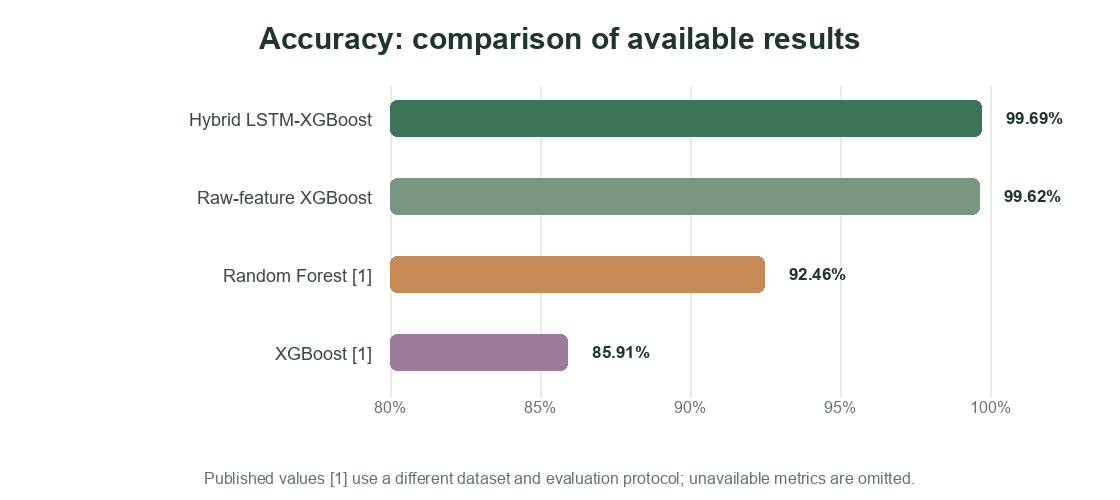
\includegraphics[width=\columnwidth]{../figures/metric_accuracy.png}\caption{Accuracy comparison.}\label{fig:metric-accuracy}\end{figure}

\begin{figure}[!t]\centering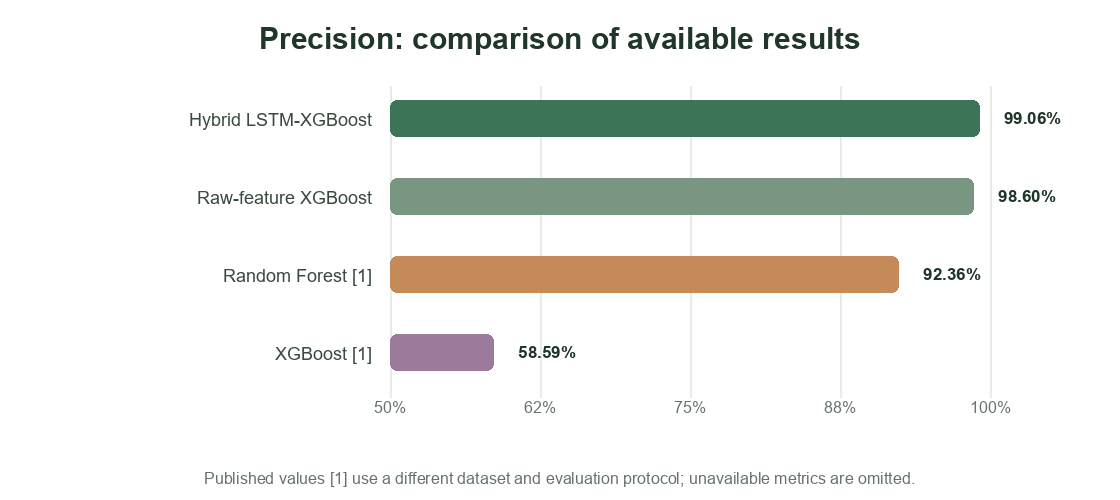
\includegraphics[width=\columnwidth]{../figures/metric_precision.png}\caption{Precision comparison.}\label{fig:metric-precision}\end{figure}

\begin{figure}[!t]\centering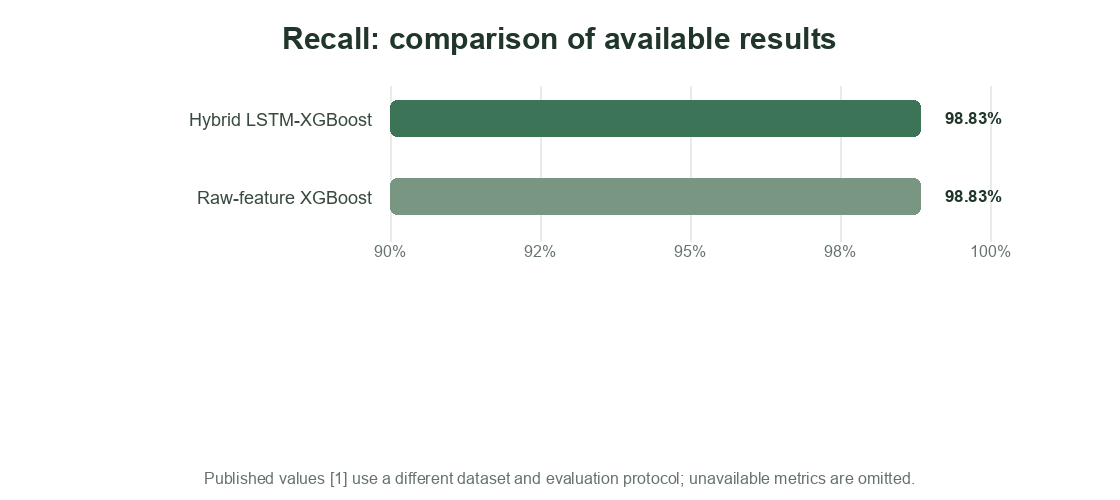
\includegraphics[width=\columnwidth]{../figures/metric_recall.png}\caption{Recall comparison.}\label{fig:metric-recall}\end{figure}

\begin{figure}[!t]\centering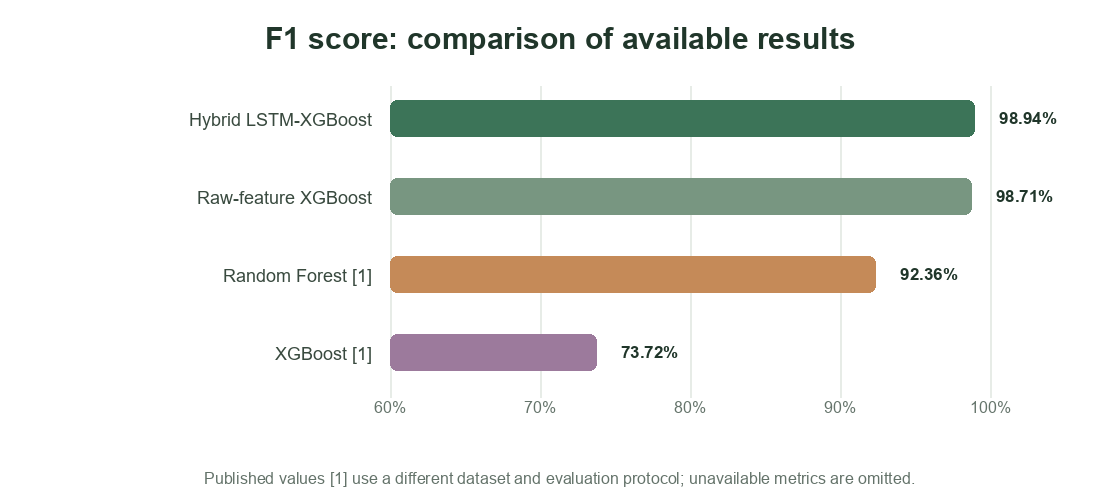
\includegraphics[width=\columnwidth]{../figures/metric_f1.png}\caption{F1 comparison.}\label{fig:metric-f1}\end{figure}

\begin{figure}[!t]\centering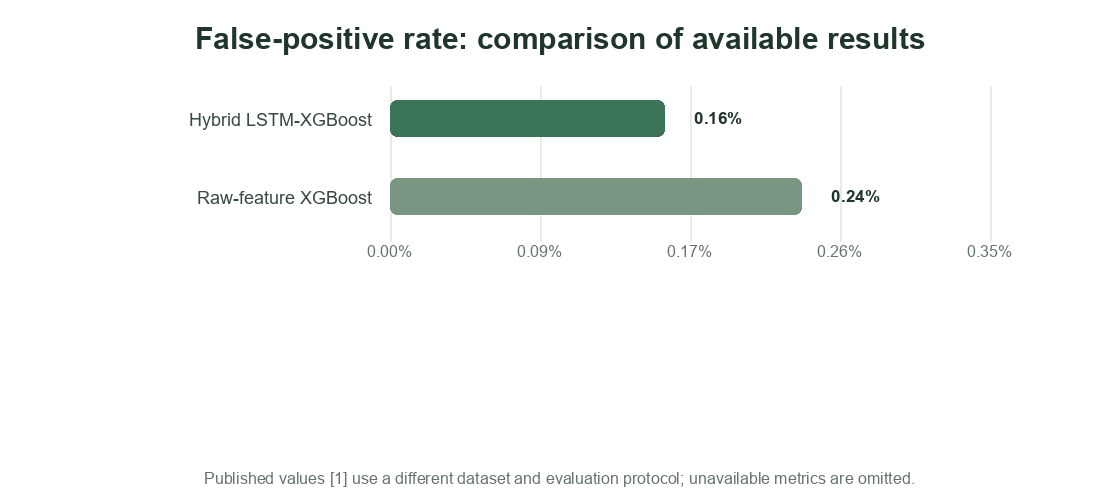
\includegraphics[width=\columnwidth]{../figures/metric_fpr.png}\caption{False-positive rate comparison.}\label{fig:metric-fpr}\end{figure}

\begin{figure}[!t]\centering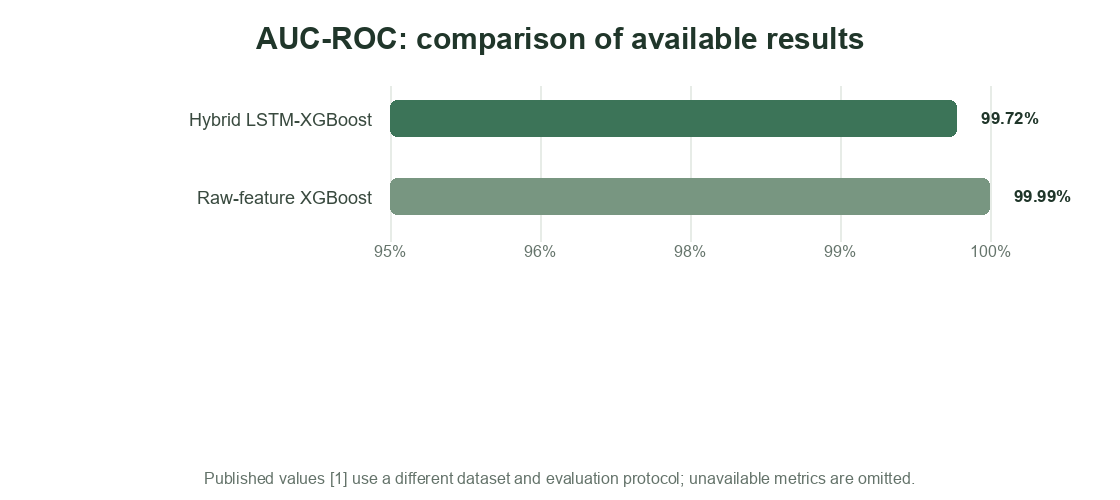
\includegraphics[width=\columnwidth]{../figures/metric_auc_roc.png}\caption{AUC-ROC comparison.}\label{fig:metric-auc_roc}\end{figure}

\begin{table}[!t]\centering\caption{Confusion counts: TN, FP, FN, TP}\begin{tabular}{l r r r r}\toprule Model & TN & FP & FN & TP \\\midrule Hybrid & 2459 & 4 & 5 & 422 \\ Raw XGBoost & 2457 & 6 & 5 & 422 \\\bottomrule\end{tabular}\end{table}

\begin{table}[!t]\centering\caption{Top XGBoost embedding importances}\begin{tabular}{r l r}\toprule Rank & Embedding & Importance \\\midrule 1 & 4 & 0.318817 \\ 2 & 10 & 0.238261 \\ 3 & 5 & 0.173671 \\ 4 & 8 & 0.117895 \\ 5 & 15 & 0.105096 \\\bottomrule\end{tabular}\end{table}

\section{Discussion}

Cow-level partitioning is useful because it avoids placing a given synthetic animal in both training and test sets. It is a stronger test of transfer to unseen cow identifiers than a random row split. It still does not create a meaningful farm-level external validation: all cows share the same generator, label rule, noise assumptions, and feature ranges.

The reported scores are expected to be optimistic. The generator samples the label first and explicitly shifts multiple sensor features conditional on that label. A model can learn those constructed differences, and a high score confirms that the code reproduces them. This does not show that the same signals reliably identify naturally occurring illness. The raw-feature baseline's very high AUC alongside a slightly lower thresholded F1 also illustrates why a single metric is insufficient.

A next study should collect prospectively timestamped collar readings, document sensor calibration and missingness, obtain outcome labels reviewed by veterinary staff, and define a cow- and preferably farm-held-out evaluation before fitting. The data split, class prevalence, threshold, and confidence intervals should be reported. For an operational dashboard, alert thresholds and user actions should be validated with farmers and veterinary partners, with a clear route for human review.

The principal result is that the requested pipeline can be executed from generation through evaluation and connected to a readable dashboard. The numeric result is not that the model is ready to detect disease. The generator builds a strong association between the label and several measurements before model fitting. This creates an easy signal for both the hybrid and raw-feature models. The held-out cows do not remove that association because train and test records come from the same set of rules.

The comparison also shows why feature importance needs context. The five largest hybrid-stage XGBoost importances correspond to embedding dimensions. An embedding index such as dimension four has no direct clinical meaning by itself. It summarizes information produced by the recurrent encoder and can mix several original variables. Interpreting these rankings as evidence that a particular sensor is clinically important would be incorrect. A future real-data study could use permutation importance at the raw input level, SHAP values with careful background selection, and ablations that remove one sensor family at a time.

The class distribution was fixed near the requested 15\% prevalence, while test prevalence is 14.78\% after sequence construction and the cow-held-out split. This small difference is expected because each cow contributes a different number of windows and the split is by identifier. Reporting both row-level and window-level prevalence prevents the two denominators from being confused. For a deployment study, prevalence should be measured from the intended farm and observation interval rather than assumed from this generator.

Before field evaluation, the data collection protocol should define sampling frequency, device placement, calibration checks, missing-data handling, and synchronization to veterinary records. Label timing matters: a measurement window must precede the event it is intended to predict, and records after treatment should not leak into training. Outcomes should specify disease and reference standard. The analysis plan should be preregistered or fixed before final testing, with farms held out when the intended use is transfer across farms.

Operational success should also be measured in terms that matter to workers: alert volume per herd-day, time from signal to review, proportion of alerts that lead to an examination, and user response. The cost of an alert depends on how often staff can check cows and whether follow-up is available. A model with acceptable discrimination could still fail if it sends too many alerts or if its output is hard to interpret. The dashboard should therefore present a reason for review, a timestamp, and a path to record a human decision, while avoiding an automated diagnosis label.

The main engineering lesson is to preserve the boundary between a demonstration and an evidence claim. In the software demonstration, a high score can confirm that preprocessing, tensor shapes, training, and evaluation execute as expected. In a research claim, that score would need to reflect independent outcomes and a test population aligned with intended use. The two purposes are both legitimate, but they require different language and different validation. This manuscript reports the former and outlines what is needed for the latter.

A future experimental design should start by defining the event horizon. If the goal is to prompt examination during the next shift, labels and feature windows must be aligned to that time horizon. Data recorded after a diagnosis or treatment may encode information that would not have been available at the time of prediction. Excluding post-event observations and defining an appropriate gap between training and test periods can reduce temporal leakage. For transfer across farms, the farm rather than the row or cow should be the held-out unit.

Researchers should also evaluate uncertainty. A single aggregate metric does not show how results vary across cows, farms, seasons, or disease categories. Bootstrap intervals can be calculated by sampling at the cow or farm level rather than treating overlapping windows as independent. This matters because neighboring windows from one cow share context and can produce correlated errors. The current paper reports counts for one cow split and does not estimate a confidence interval; its precise percentages should not be mistaken for high precision about future performance.

Fair comparison requires a shared evaluation manifest. Every candidate model should receive the same training cows, validation strategy, and test cows. If one model uses SMOTE and another does not, both choices should be evaluated as separate factors in a factorial experiment. Thresholds should be chosen only on validation data, then frozen before test evaluation. Hyperparameter search should be documented, and the test set should not be repeatedly inspected to choose the best configuration. Such controls would make it possible to attribute an observed difference to the model or training strategy rather than to a protocol change.

Model outputs should be calibrated if they are displayed as probabilities. A score of 0.8 is often read as an 80\% chance, which is only justified if predicted probabilities match observed frequencies in a relevant population. Calibration plots, Brier score, and reliability measures can help evaluate that property. The present dashboard displays a heuristic percentage and explicitly does not call it the trained classifier probability. Any future integration should change that interface only after an end-to-end data contract and probability calibration have been established.

\section{Limitations And Ethics}

This is a synthetic software study. It contains no animal participants, real farm observations, or clinical diagnosis. Its target is generated, rather than adjudicated by a veterinarian. Row order is used to create three-step windows, and those steps are not dated observations. Temperature, pulse, activity, rumination, gait, ventilation, and forage are simplified distributions, not calibrated sensor models. The dashboard feed is also synthetic and its heuristic score is not the classifier output.

The test set contains one split of 45 cows and 2,890 sequence windows. The paper reports no repeated-seed confidence interval, prospective trial, external farm evaluation, or device-latency measurement. Feature importance for the hybrid XGBoost stage refers to learned embedding dimensions, not directly to interpretable sensor variables. Synthetic performance should not guide treatment decisions, and the interface should not be connected to clinical workflows until data governance, security, veterinary oversight, and validation are in place.

There are several additional limitations. First, the observed 10,000-row file is produced by code and is not a sample from a commercial dairy. Second, the fixed random seed makes the result reproducible but does not characterize variation across seeds. Third, windows are constructed from row order and not from validated temporal trajectories. Fourth, synthetic measurements are not calibrated against specific collar hardware. Fifth, only one train-test partition is reported. Sixth, the comparator configurations differ in resampling and feature representations, so their score difference cannot be attributed solely to the LSTM.

An ethically responsible next step would collect data under an approved farm protocol, obtain consent from farm operators where required, minimize personal information, and define who can access animal records. Animal health decisions should remain under qualified human oversight. The dashboard should label uncertain alerts as prompts for review and preserve enough context to support that review. A model should not recommend treatment or replace veterinary examination on the basis of a generated score.

The evaluation should be expanded with multiple farms, repeated temporal splits, uncertainty intervals, and subgroup analyses where the sample size supports them. Calibration should be assessed on a naturally imbalanced holdout, and the alert threshold should be selected using a documented trade-off between missed cases and false alarms. External validation should be completed before any prospective workflow pilot. Monitoring after deployment would need to detect sensor drift, changes in disease prevalence, and data pipeline failures.

A practical validation sequence can begin with a silent prospective phase. During this phase, devices collect time-stamped readings and the model produces scores that are hidden from farm staff. Veterinary reviewers can then compare flagged windows with the agreed clinical reference standard without allowing the score to change care. This design helps estimate sensitivity, false-alert burden, missingness, and score calibration before an alert is introduced into daily work. It also reveals whether measurement coverage is adequate during the periods when an early warning is intended.

After the silent phase, a limited workflow pilot can test whether alerts are understandable and actionable. The pilot should record when a worker opens an alert, whether an examination follows, and the outcome of that examination. A safety review should examine missed cases and false alarms, not only aggregate accuracy. Stop criteria should be defined in advance for device failures, excessive alert load, or evidence that the interface is being mistaken for a diagnosis. Farm staff should be able to report confusing signals and disable the feed if the service becomes unreliable.

For reproducible reporting, each model version should be tied to a data snapshot, feature definition, split manifest, training configuration, threshold, and code revision. The test set must remain protected until the comparison is finalized. If repeated model tuning uses the same holdout, it gradually becomes part of the development process and its score becomes optimistic. A later external test should therefore be collected from a different time period or farm and evaluated once under the locked protocol.

The result is limited to a single seed and a single partition of cow identifiers. It does not estimate between-farm variation, seasonal change, device replacement, or rare disease performance. No confidence intervals are reported. The minority class contains 427 test windows, but those windows may not represent independent disease episodes because adjacent windows can overlap. The synthetic ordering does not represent real temporal dependence, and the same generation rules create both training and test records.

The study is not a clinical trial, an animal experiment, or a validated diagnostic study. No animal health record is included in the distributed CSV. Labels are generated and measurements are simulated. The dashboard feed is also synthetic and its heuristic does not use the trained model. These distinctions should travel with the files if the package is shared or copied to a repository. A screenshot or chart without its caveat could otherwise be misread as farm evidence.

Data governance for a future farm study should cover ownership, retention, access, and deletion. Cow identifiers may appear non-personal, but linked records can reveal farm operations and commercial practices. Access should follow least privilege, credentials should not be committed to a repository, and data exports should be reviewed before sharing. The public demonstration contains no private farm records and does not provide authentication. A real deployment should receive a security review before accepting production data.

Finally, livestock monitoring can affect human work as well as animal care. A system that produces frequent false alarms can interrupt routines and reduce trust. A system that hides uncertainty can lead users to over-rely on a score. Participatory design with farmers and veterinary staff should examine wording, alert timing, workload, and escalation paths. The intended role of the model should be stated in training materials and within the interface, and users should have a straightforward way to report errors or suspend alerts.

\section{Conclusion}

This work turns a collar-inspired monitoring idea into a reproducible synthetic benchmark and a farmer/admin dashboard prototype. The hybrid LSTM-XGBoost model achieved 99.69\% accuracy and 98.94\% F1 on a cow-held-out synthetic test set, while a raw-feature XGBoost comparator achieved 99.62\% accuracy and 98.71\% F1. Because the generator encodes the target into the sensor distributions, these values describe the synthetic data experiment rather than a real disease-detection capability. The practical next step is not to deploy the scores, but to replace the synthetic data generator with timestamped farm data and evaluate the complete sensing, prediction, alert, and review workflow under veterinary supervision.

The work provides a complete, reproducible software demonstration: a 10,000-row dataset, a cow-held-out sequence experiment, a hybrid classifier, a raw-feature comparator, a metric report, and a farmer-facing interface. It also makes the main limitation explicit: the measured scores reflect label-dependent data generation. The dashboard is a simulated preview, and its risk indicator is not the trained model's output.

The next scientific step is to replace the generator with timestamped observations and veterinarian-reviewed outcomes, then evaluate the frozen pipeline on cows and farms that were not used during development. Only after that step can researchers estimate whether the signals, metrics, and alert workflow transfer to livestock care. Until then, the current artifacts are intended for code review, teaching, and interface exploration rather than farm decisions.

\begin{thebibliography}{9}

\bibitem{ref1} Kaur, D., \& Virk, A. K. (2025). Smart neck collar: IoT-based disease detection and health monitoring for dairy cows. Discover Internet of Things, 5, Article 12. \url{https://doi.org/10.1007/s43926-025-00109-5}

\bibitem{ref2} Chawla, N. V., Bowyer, K. W., Hall, L. O., \& Kegelmeyer, W. P. (2002). SMOTE: Synthetic minority over-sampling technique. Journal of Artificial Intelligence Research, 16, 321-357. \url{https://doi.org/10.1613/jair.953}

\bibitem{ref3} Hochreiter, S., \& Schmidhuber, J. (1997). Long short-term memory. Neural Computation, 9(8), 1735-1780. \url{https://doi.org/10.1162/neco.1997.9.8.1735}

\bibitem{ref4} Chen, T., \& Guestrin, C. (2016). XGBoost: A scalable tree boosting system. Proceedings of the 22nd ACM SIGKDD International Conference on Knowledge Discovery and Data Mining, 785-794. \url{https://doi.org/10.1145/2939672.2939785}

\bibitem{ref5} Fawcett, T. (2006). An introduction to ROC analysis. Pattern Recognition Letters, 27(8), 861-874. \url{https://doi.org/10.1016/j.patrec.2005.10.010}

\bibitem{ref6} Saito, T., \& Rehmsmeier, M. (2015). The precision-recall plot is more informative than the ROC plot when evaluating binary classifiers on imbalanced datasets. PLOS ONE, 10(3), e0118432. \url{https://doi.org/10.1371/journal.pone.0118432}

\bibitem{ref7} He, H., \& Garcia, E. A. (2009). Learning from imbalanced data. IEEE Transactions on Knowledge and Data Engineering, 21(9), 1263-1284. \url{https://doi.org/10.1109/TKDE.2008.239}

\bibitem{ref8} Roberts, D. R., Bahn, V., Ciuti, S., Boyce, M. S., Elith, J., Guillera-Arroita, G., Hauenstein, S., Lahoz-Monfort, J. J., Schröder, B., Thuiller, W., Warton, D. I., Wintle, B. A., Hartig, F., \& Dormann, C. F. (2017). Cross-validation strategies for data with temporal, spatial, hierarchical, or phylogenetic structure. Ecography, 40(8), 913-929. \url{https://doi.org/10.1111/ecog.02881}

\bibitem{ref9} Collins, G. S., Reitsma, J. B., Altman, D. G., \& Moons, K. G. M. (2015). Transparent Reporting of a multivariable prediction model for Individual Prognosis Or Diagnosis (TRIPOD): The TRIPOD Statement. Journal of Clinical Epidemiology, 68(2), 134-143. \url{https://doi.org/10.1016/j.jclinepi.2014.11.010}

\bibitem{ref10} Van Calster, B., McLernon, D. J., van Smeden, M., Wynants, L., \& Steyerberg, E. W. (2019). Calibration: the Achilles heel of predictive analytics. BMC Medicine, 17, 230. \url{https://doi.org/10.1186/s12916-019-1466-7}

\bibitem{ref11} Cerri, R. L. A., Burnett, T. A., Madureira, A. M. L., Silper, B. F., Denis-Robichaud, J., LeBlanc, S., Cooke, R. F., \& Vasconcelos, J. L. M. (2021). Symposium review: Linking activity-sensor data and physiology to improve dairy cow fertility. Journal of Dairy Science, 104(1), 1220-1231. \url{https://doi.org/10.3168/jds.2019-17893}

\bibitem{ref12} Kang, X., Zhang, X. D., \& Liu, G. (2021). A Review: Development of Computer Vision-Based Lameness Detection for Dairy Cows and Discussion of the Practical Applications. Sensors, 21(3), 753. \url{https://doi.org/10.3390/s21030753}

\bibitem{ref13} O'Leary, N. W., Byrne, D. T., O'Connor, A. H., \& Shalloo, L. (2020). Invited review: Cattle lameness detection with accelerometers. Journal of Dairy Science, 103(5), 3895-3911. \url{https://doi.org/10.3168/jds.2019-17123}

\bibitem{ref14} Rutten, C. J., Velthuis, A. G. J., Steeneveld, W., \& Hogeveen, H. (2013). Invited review: Sensors to support health management on dairy farms. Journal of Dairy Science, 96(4), 1928-1952. \url{https://doi.org/10.3168/jds.2012-6107}

\bibitem{ref15} Hendriks, S. J., Phyn, C. V. C., Huzzey, J. M., Mueller, K. R., Turner, S., Donaghy, D. J., \& Roche, J. R. (2020). Graduate Student Literature Review: Evaluating the appropriate use of wearable accelerometers in research to monitor lying behaviors of dairy cows. Journal of Dairy Science, 103(12), 12140-12157. \url{https://doi.org/10.3168/jds.2019-17887}

\bibitem{ref16} Lora, I., Gottardo, F., Contiero, B., Zidi, A., Magrin, L., Cassandro, M., \& Cozzi, G. (2020). A survey on sensor systems used in Italian dairy farms and comparison between performances of similar herds equipped or not equipped with sensors. Journal of Dairy Science, 103(11), 10264-10272. \url{https://doi.org/10.3168/jds.2019-17973}

\bibitem{ref17} Stone, A. E. (2020). Symposium review: The most important factors affecting adoption of precision dairy monitoring technologies. Journal of Dairy Science, 103(6), 5740-5745. \url{https://doi.org/10.3168/jds.2019-17148}

\bibitem{ref18} Grinter, L. N., Campler, M. R., \& Costa, J. H. C. (2019). Technical note: Validation of a behavior-monitoring collar's precision and accuracy to measure rumination, feeding, and resting time of lactating dairy cows. Journal of Dairy Science, 102(4), 3487-3494. \url{https://doi.org/10.3168/jds.2018-15563}

\end{thebibliography}

\end{document}